% document came from
%	https://publishingsupport.iopscience.iop.org/questions/latex-template/
% via 
% 	https://publishingsupport.iopscience.iop.org/journals/physics-education/
\documentclass[12pt]{iopart}
%
\usepackage{graphicx} % needed for figures
%\usepackage{float}
%\usepackage{units}
%\usepackage{hyperref}

\newcommand{\be}{\begin{equation}}
\newcommand{\ee}{\end{equation}}
\newcommand{\bea}{\begin{eqnarray}}
\newcommand{\eea}{\end{eqnarray}}
\newcommand{\degC}{^{\circ}C}
%

\begin{document}
\title[Using Open Source Intelligence Techniques to evaluate Physics Calculations]{Using Open Source Intelligence Techniques to evaluate Physics Calculations}

\author{Nathan T. Moore}

\address{
	Physics and General Engineering, 
	Winona State University,
	Winona, MN 55987 USA
}
\ead{nmoore@winona.edu}
\vspace{10pt}
\begin{indented}
\item[\today]
\end{indented}

\begin{abstract}
Checking the answer at the end of a calculation is an oft neglected part of a calculation, and getting students to engage in this behavior can be difficult when they are already intellectually tired. 
	The paper briefly describes a graphing, linearization, and control of variables activity related to pendulums, couched as ``swingset" design. 
	After a reliable $swingtime \sim \sqrt{length}$ model has been established, students apply the model to a youtube video to predict the height of a bridge. 
	Then, to reinforce the ideas of multiple representations, and multiple lines of evidence within an argument, students are asked to use Google Maps and other online resources to estimate the height of the bridge. 
	Looking for overlap between online estimations and physical models from the lab is powerful. 
	At the end of the exercise, students have had a brief introduction to ``Open Source Intelligence" techniques that are commonly used by news and intelligence organizations. 
\end{abstract}

%
% Uncomment for keywords
%\vspace{2pc}
%\noindent{\it Keywords}: XXXXXX, YYYYYYYY, ZZZZZZZZZ
%
% Uncomment for Submitted to journal title message
%\submitto{\JPA}
%
% Uncomment if a separate title page is required
%\maketitle
% 
% For two-column output uncomment the next line and choose [10pt] rather than [12pt] in the \documentclass declaration
%\ioptwocol
%



\section{Swingset Exercise}
Early in a Physical Science or Introductory Physics-Mechanics class, we introduce and practice control of variables, graphing, and linearization concepts by asking students to think about designing a new swingset for an elementary school playground.  
An exciting swingset takes a long time to swing back and forth and we call this ``swingtime" the output variable we want to be able to predict.
Formally, a swingset is typically modeled as a pendulum with period 
$T \sim \sqrt{L}$ \cite{openstax_pendulum} but as this activity usually occurs in the first few weeks of the class, we avoid using this distracting technical jargon.

\begin{figure}[h]
\centering
        %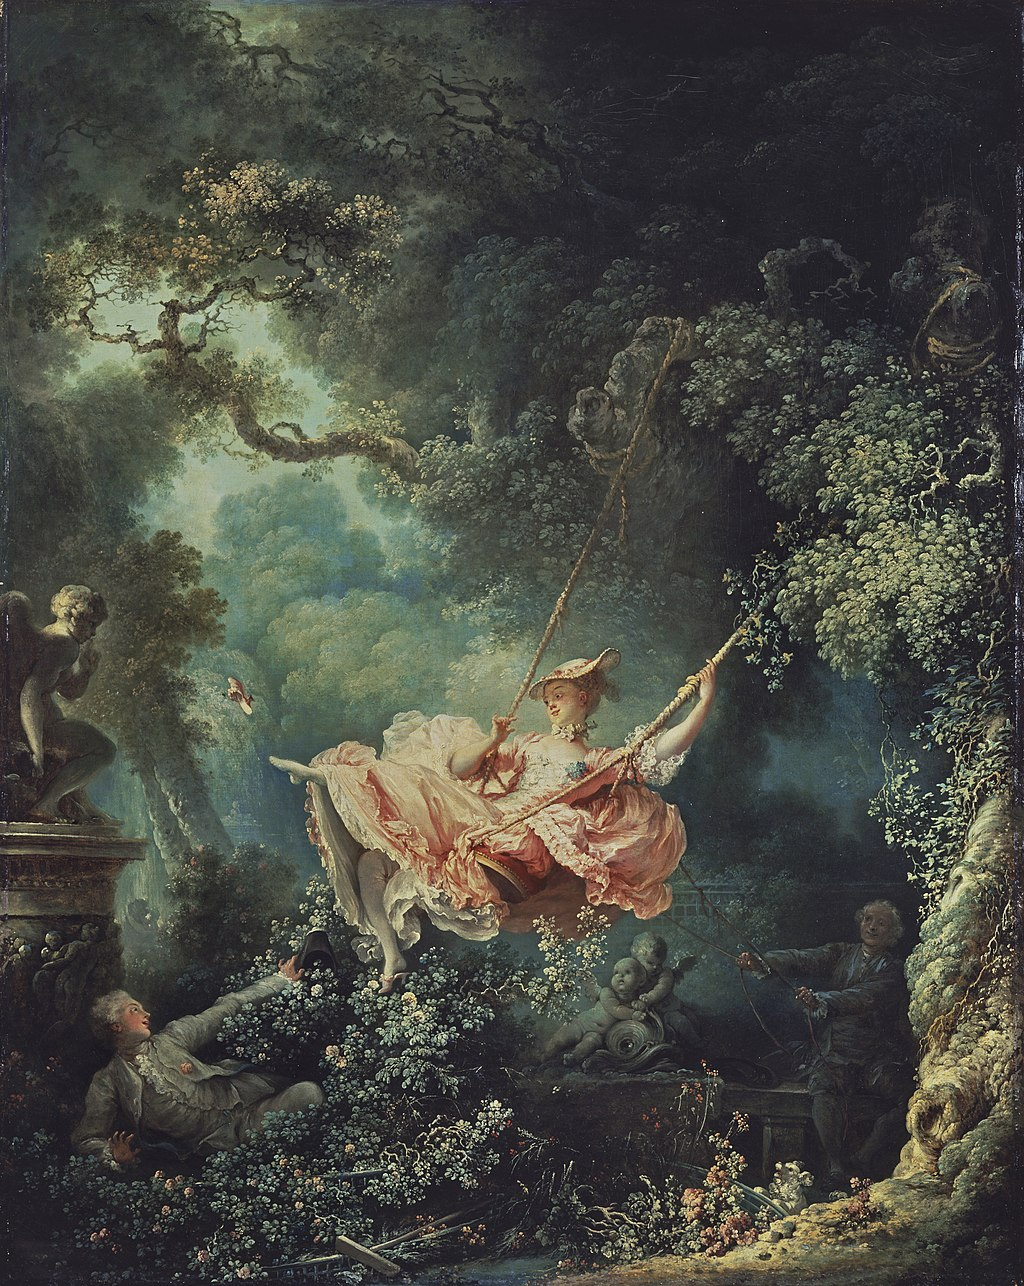
\includegraphics[width=\columnwidth]{Fragonard,_The_Swing.jpg}
        %\includegraphics[width=\columnwidth]{2023-05-01.pdf}
        %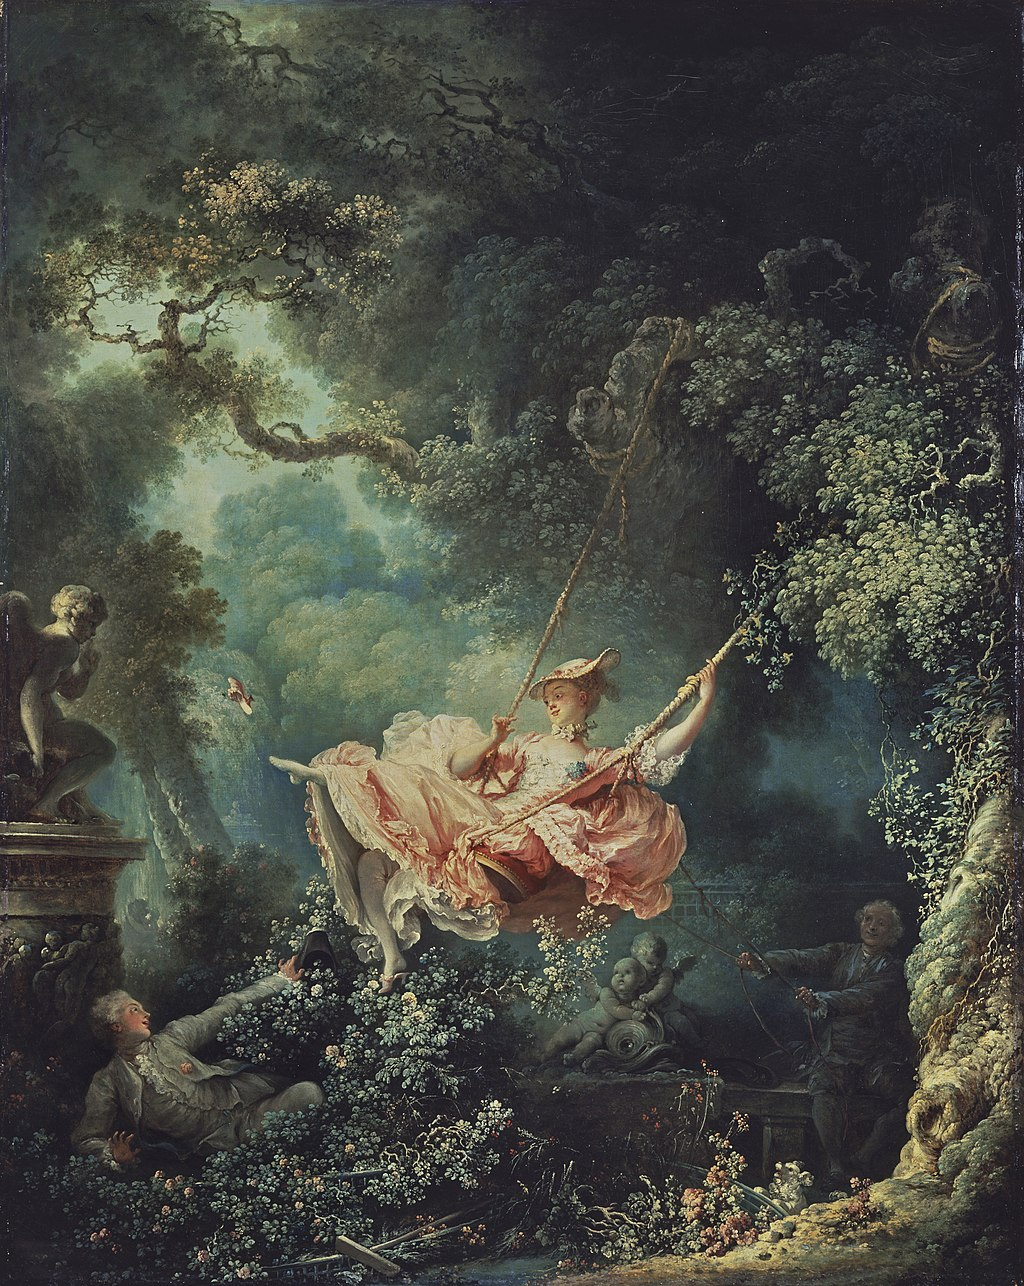
\includegraphics[]{Fragonard,_The_Swing.jpg}
\caption{
In North America, a ``swingset" or ``swing" is a mass-rope pendulum system that people enjoy using.
        Swings have a long history of recreational use throughout many human cultures \cite{swings-wikipedia}.
}
\label{buffet}
\end{figure}

When asked about possible input variables on which swingtime might depend, students will often talk about mass, weight, initial height and angle, whether you start from rest or with an initial push, and length.  
After breif investigations, the students typically settle on initial angle, mass, and length as the most important variables needed to predict swingtime.  
With further data collection, the class can narrow down the length of the swing's cable as the most important variable.  

\begin{figure}[h]
\centering
        %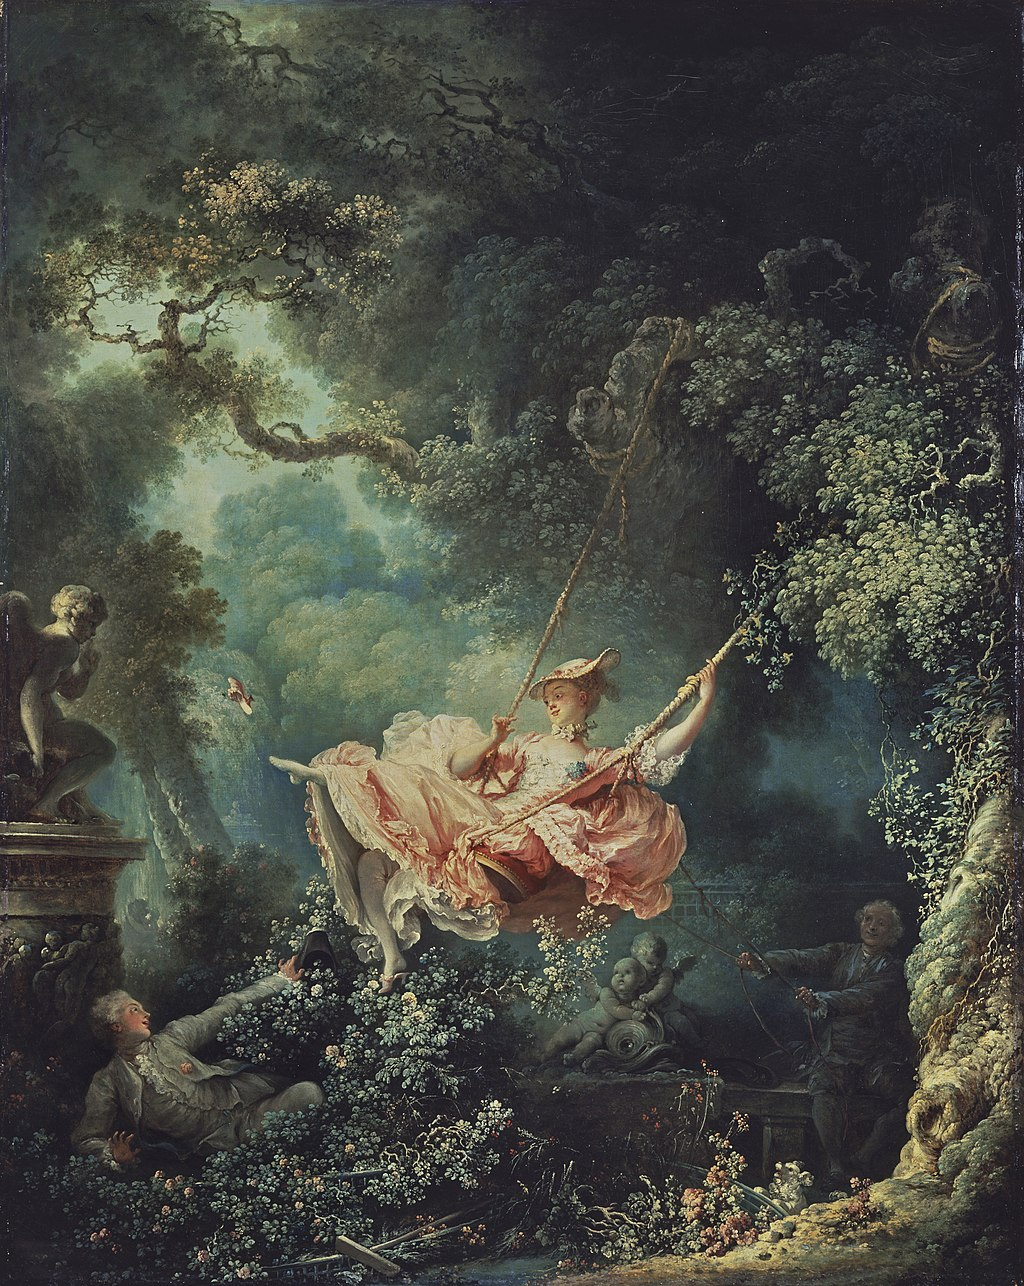
\includegraphics[width=\columnwidth]{Fragonard,_The_Swing.jpg}
        %\includegraphics[width=\columnwidth]{2023-05-01.pdf}
        %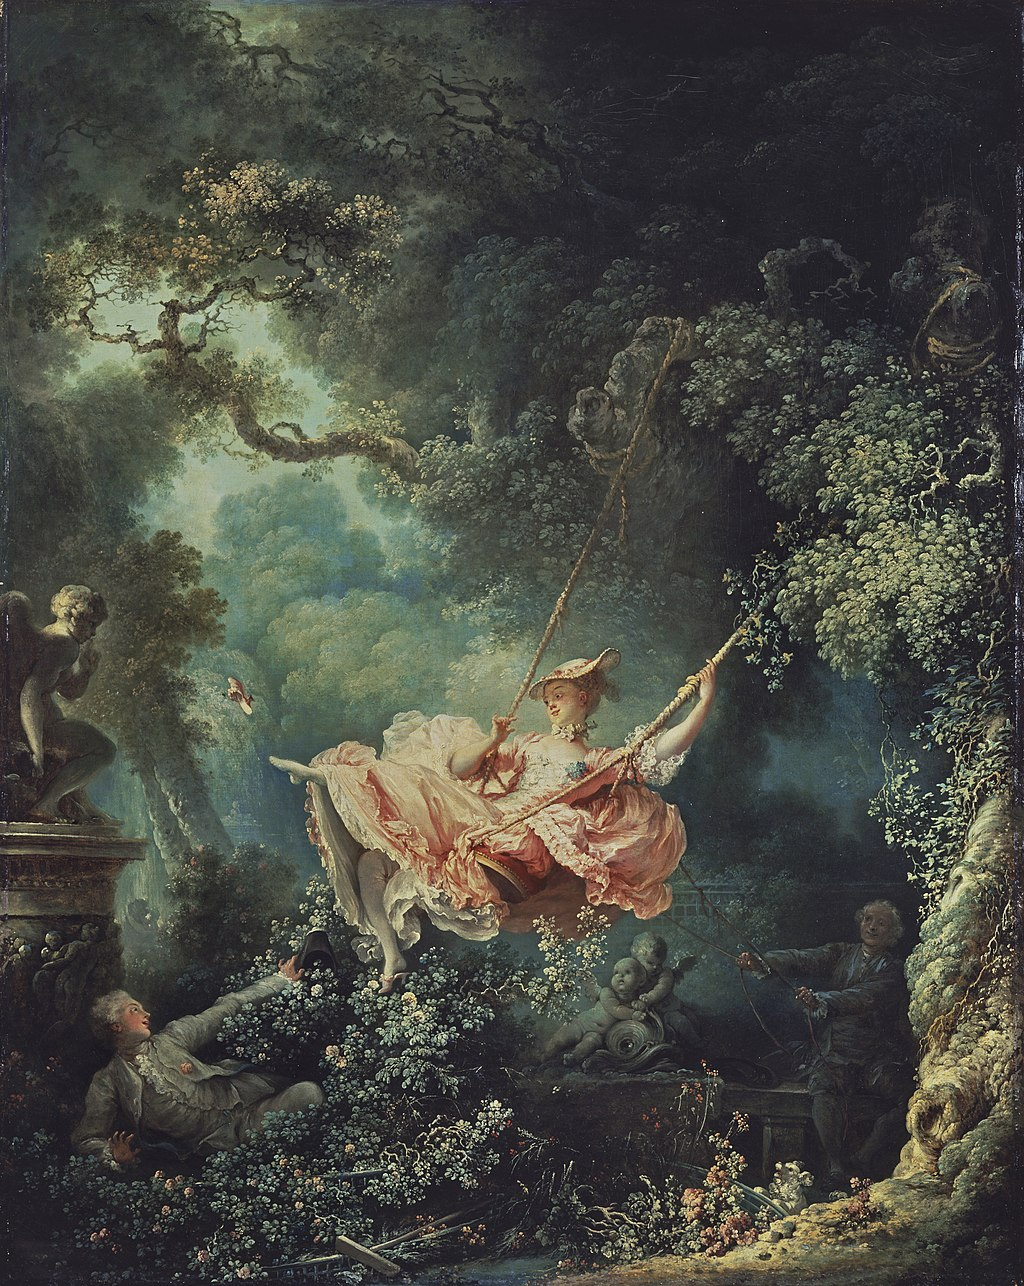
\includegraphics[]{Fragonard,_The_Swing.jpg}
\caption{
Typical student data, using metal washers and string to model the motion of a swingset.
        Students are coached to measure the time associated with multiple ``there and back" swings and then divide to find an average time so that their reaction times (typically $\approx0.3 seconds$) can be ignored.
        }
        \label{swingtime_graph}
\end{figure}

Data from a past class is given in figure \ref{swingtime_graph}. Thus far, all of the students' data has been collected with metal washers and string, with none of the model swingsets greater than about $100cm$ in length. The data in figure \ref{swingtime_graph} looks fairly linear, and when asked  to predict the swingtime for a $200cm$ length, students typically either draw a line or use a linear math model.  

As seen, the linear model fails at longer lengths. Resolution comes via two pieces of data.  First, if a swingset has ``almost no length" students will generally volunteer that it takes ``almost no time" to swing back and forth.  This means that the length=0, swingtime=0 intercept is physically real and should be included in fitting efforts.  

Second, when the $200cm$ and $500cm$ points are included in the graph, students can be coached to reccollect that the data reminds them of a parabola that has been rotated to open towards the positive x-axis of the graph.  In Pre-Calculus or Algebra 2 this mathematical form is often written as a $y^2=x$ or $y=\sqrt{x}$ relationship.  

This discussion is implemented in a linearized graph, seen in figure \ref{linearized_swingtime_graph}. 

\begin{figure}[h]
\centering
	%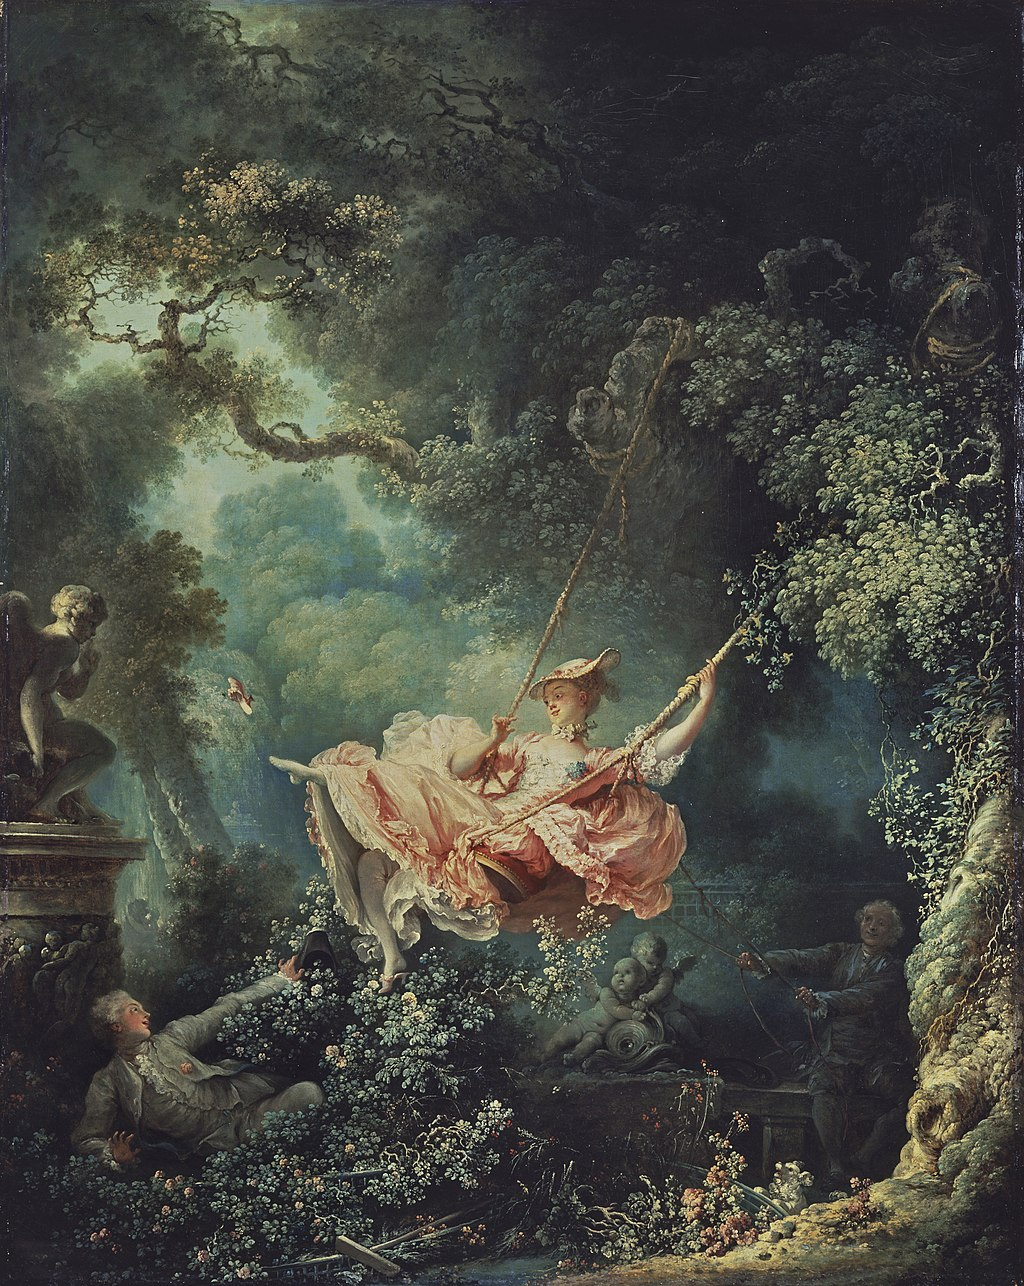
\includegraphics[width=\columnwidth]{Fragonard,_The_Swing.jpg}
\caption{
	Linearized swingset data from a class.  Note that $200cm$ and $500cm$ lengths are included and described well bu the trendline.  The ``almost no length" swingset that takes ``almost no time" to swing is also nicely included.   
	}
	\label{linearized_swingtime_graph}
\end{figure}


Thus far the 

\subsection{predicting youtube video height}


\section{Evaluating answer using Open Source Intelligence}

\subsection{screen grab and scaling}

\subsection{geographic searching}
- wrong bridge in Sault St. Marie

\subsection{shadows}

\subsection{geographic clues}
Moab arches

\clearpage
\section*{References}
\begin{thebibliography}{99}

\bibitem{openstax_pendulum}
College Physics 2e
16.4 The Simple Pendulum
https://openstax.org/books/college-physics-2e/pages/16-4-the-simple-pendulum

\bibitem{the_swing_Fragonard}
	https://commons.wikimedia.org/wiki/File:Fragonard,\_The\_Swing.jpg
	Jean-Honoré Fragonard: The Swing 
	1767

\bibitem{swings-wikipedia}
	https://en.wikipedia.org/wiki/Swing\_(seat)
		Swing (seat)

\end{thebibliography}


\end{document}

